\section{Input-to-State Stable (ISS) Coupled Oscillator Networks (CONs)}\label{sec:con:con}

\subsection{Formulation} 
The integral component to (coupled) oscillatory \glspl{RNN}~\cite{rusch2020coupled, rusch2021unicornn, ceni2024random, lanthaler2024neural} are one-dimensional, potentially damped, harmonic oscillators, which are described by their state $y_i = \begin{bmatrix}
    x_i & \dot{x}_i
\end{bmatrix}^\mathrm{T} \in \mathbb{R}^2$, where $x_i$ and $\dot{x}_i$ are the position and velocity of the oscillator, respectively. Then, the oscillator's dynamics are defined by the following \gls{EOM}
\begin{equation}\label{eq:con:harmonic_oscillator}
    m_i \, \ddot{x}_i(t) + d_i \, \dot{x}_i(t) + \kappa_i \, x_i(t) = F_i(t),
    \qquad
    \text{with } m_i, \kappa_i, d_i \in \mathbb{R}^+.
\end{equation}
Here, $m_i$ is the mass, $\kappa_i$ is the stiffness, and $d_i$ is the damping coefficient of the damped harmonic oscillator. $F_i(t) \in \mathbb{R}$ is a (possibly time-dependent) external forcing term acting on the mass.

Even though the state is extremely low dimensional and the number of parameters is small, this single, damped harmonic oscillator can already exhibit a variety of (designable) behaviors:
The expressions $\omega_{\mathrm{n},i} = \sqrt{\frac{\kappa_i}{m_i}}$ and $\zeta_i = \frac{d_i}{2 \, \sqrt{\kappa_i \, m_i}}$ let us determine the natural frequency and the damping factor, respectively and allow us to design the transient behavior. For example, $\omega_{\mathrm{n},i}$ lets us isolate a spectrum of the input signal $F_i(t)$~\cite{ceni2024random} and $\zeta_i$ determines the damping regime: underdamped ($\omega_{\mathrm{n},i} < 1$), critically damped ($\omega_{\mathrm{n},i} = 1$), overdamped ($\omega_{\mathrm{n},i} > 1$). 
Furthermore, as (damped) harmonic oscillators are omnipresent in nature (and especially in physical systems), they have been intensively studied and are well understood (e.g., characteristics, closed-form solutions, etc.). 
In this work, we will exploit some of these properties and knowledge to learn stable (latent) dynamics efficiently.

By intercoupling damped harmonic oscillators, we can drastically increase the expressiveness of the dynamical system~\cite{rusch2020coupled, ceni2024random, lanthaler2024neural} while preserving some of the intuition and understanding we have for these systems. In this work, we propose a \gls{ISS}-stable \gls{CON} consisting of $n$ damped harmonic oscillators that are coupled through both linear and nonlinear terms. The networks' state is defined as $y = \begin{bmatrix}
    x^\mathrm{T} & \dot{x}^\mathrm{T}
\end{bmatrix}^\mathrm{T} \in \mathbb{R}^{2n}$ and its dynamics can be formulated as a \nth{2}-order \gls{ODE}
\begin{equation}\label{eq:con:con_dynamics}
    \dot{y}(t) = \begin{bmatrix}
        \frac{\mathrm{d}x}{\mathrm{d}t}\\
        \frac{\mathrm{d}\dot{x}}{\mathrm{d}t}
    \end{bmatrix} = f(y(t), u(t)) = \begin{bmatrix}
        \dot{x}(t)\\
        g(u(t)) -K x(t) - D \, \dot{x}(t) - \tanh(W \, x(t) + b)
    \end{bmatrix},
\end{equation}
where $K, D \in \mathbb{R}^{n \times n}$ are the linear stiffness and damping matrices, respectively. The neuron-inspired term $\tanh(W \, x(t) + b)$ with $W \in \mathbb{R}^{n \times n}$, $b \in \mathbb{R}^n$ provides nonlinear coupling between the harmonic oscillators.
The network is excited by the time-dependent input $u(t) \in \mathbb{R}^m$ through the possibly nonlinear mapping $g: \mathbb{R}^m \to \mathbb{R}^n$.
Specifically, we consider in this work a formulation where an input-dependent matrix $B(u) \in \mathbb{R}^{n \times m}$ projects the input $u(t)$ to a time-dependent forcing on the oscillators: $\tau = g(u) = B(u) \, u$. Here $B(u)$ could, for example, be parametrized by a \gls{MLP}.

We specifically designed the network architecture such that (i) the system exhibits a unique and isolated equilibrium and (ii) we can derive expressions for the kinetic and potential energies. These two features allow us to (a) prove \gls{GAS} and \gls{ISS} stability using an established procedure based on strict Lyapunov arguments~\cite{calzolari2020exponential, wu2022passive}, and (b) implement model-based controller based on potential shaping.

\subsection{Potential energy and determination of equilibria}

One key insight of this work is that in the coordinates $x(t), \dot{x}(t)$, we cannot derive a potential 
% and subsequently use Lyapunov arguments to prove stability 
as the hyperbolic force $\tanh(W x(t) + b)$ is not symmetric. Therefore, we propose a coordinate transformation into $\mathcal{W}$-coordinates: $y_\mathrm{w}(t) = \begin{bmatrix}
    x_\mathrm{w}(t)\\
    \dot{x}_\mathrm{w}(t)\\
\end{bmatrix} = \begin{bmatrix}
    W \, x(t)\\
    W \, \dot{x}(t)
\end{bmatrix} \in \mathbb{R}^{2n}$. The coordinate transformation is valid if its Jacobian is full-rank, which is the case if $\mathrm{rank}(W) = n$.
In $\mathcal{W}$-coordinates, the dynamics can be rewritten as
\begin{equation}\label{eq:con:conw_dynamics}
    \dot{y}_\mathrm{w}(t) = \begin{bmatrix}
        \frac{\mathrm{d}x_\mathrm{w}}{\mathrm{d}t}\\
        \frac{\mathrm{d}\dot{x}_\mathrm{w}}{\mathrm{d}t}
    \end{bmatrix} = f_\mathrm{w}(y(t), u(t)) = \begin{bmatrix}
        \dot{x}_\mathrm{w}(t)\\
        M_\mathrm{w}^{-1} \, \left (g(u(t)) -K_\mathrm{w} x_\mathrm{w}(t) - D_\mathrm{w} \, \dot{x}_\mathrm{w}(t) - \tanh(x_\mathrm{w}(t) + b) \right )
    \end{bmatrix}
\end{equation}
with $K_\mathrm{w} = K \, W$, $D_\mathrm{w} = D \, W$ and $M_\mathrm{w} = W^{-1}$. 

A difference of this formulation compared to prior work~\cite{rusch2020coupled, rusch2021unicornn, ceni2024random, lanthaler2024neural} is that (i) the forcing produced by the input term $\tau = g(u)$ is fully separated from the forcing produced by the elastic coupling terms $K_\mathrm{w}$, and (ii) the generalized force is symmetric as stated in Lemma~\ref{lemma:con:conw_symmetric_potential}, allowing us to define a potential energy expression, which we can later on leverage for stability analysis and control.

\begin{lemma}\label{lemma:con:conw_symmetric_potential}
    Let $\tilde{x}_\mathrm{w} \in \mathbb{R}^n$ be generalized coordinates and $\bar{x}_\mathrm{w}, b \in \mathbb{R}^n$ constants.
    Then, the potential force of system \eqref{eq:con:conw_residual_dynamics}
    \begin{equation}
        \tilde{f}_{\mathcal{U}_\mathrm{w}}(\tilde{x}_\mathrm{w}) = K_\mathrm{w} (\bar{x}_\mathrm{w} + \tilde{x}_\mathrm{w}) + \tanh(\bar{x}_\mathrm{w} + \tilde{x}_\mathrm{w} + b),
    \end{equation}
    stems from the potential
    \begin{equation}
        \mathcal{U}_\mathrm{w}(\tilde{x}_\mathrm{w}) = \sum_{i=1}^n \int_{0}^{\tilde{x}_{\mathrm{w},i}} \tanh(\bar{x}_{\mathrm{w},i}+\sigma+b_i) \, \mathrm{d} \sigma - \sum_{i=1}^n \int_{0}^{\tilde{x}_{\mathrm{w},i}} \tanh(\bar{x}_{\mathrm{w},i}+b_i) \, \mathrm{d} \sigma \in \mathbb{R}.
    \end{equation}
\end{lemma}
\begin{proof}
    First, we take the derivative of $\mathcal{U}(\tilde{x}_\mathrm{w})$:
    \begin{equation}
        \frac{\partial \mathcal{U}_\mathrm{w}}{\partial \tilde{x}_\mathrm{w}} = K_\mathrm{w} (\bar{x}_\mathrm{w} + \tilde{x}_\mathrm{w}) + \tanh(\bar{x}_\mathrm{w} + \tilde{x}_\mathrm{w} + b) = \tilde{f}_{\mathcal{U}_\mathrm{w}}.
    \end{equation}
    The Hessian of the potential is given by
    \begin{equation}
        H_{\mathcal{U}_\mathrm{w}}(\tilde{x}_\mathrm{w}) = \frac{\partial^2 \mathcal{U}_\mathrm{w}}{\partial \tilde{x}_\mathrm{w}^2} = \frac{\partial \tilde{f}_{\mathcal{U}_\mathrm{w}}}{\partial \tilde{x}_\mathrm{w}}  = K_\mathrm{w} + S_\mathrm{sech}^{2}(\tilde{x}_\mathrm{w}) \in \mathbb{R}^{n \times n}.
    \end{equation}
    As $K_\mathrm{w} \succ 0 \Rightarrow K_\mathrm{w} = K_\mathrm{w}^\mathrm{T}$, we can easily show that the potential force is symmetric:
    \begin{equation}
        H_{\mathcal{U}_\mathrm{w}}^\mathrm{T} = K_\mathrm{w}^\mathrm{T}  + S_\mathrm{sech}^{2}(\tilde{x}_\mathrm{w})^\mathrm{T} = K_\mathrm{w} + S_\mathrm{sech}^{2}(\tilde{x}_\mathrm{w}) = H_{\mathcal{U}_\mathrm{w}}.
    \end{equation}
\end{proof}

The equilibria $\bar{y}_\mathrm{w} = \begin{bmatrix}
    \bar{x}_\mathrm{w}^\mathrm{T} & 0^\mathrm{T}
\end{bmatrix}^\mathrm{T} \in \mathbb{R}^{2n}$ of the unforced network are given by the roots of the characteristic equation $\tanh(\bar{x}_\mathrm{w} + b) + K_\mathrm{w} \, \bar{x}_\mathrm{w} = 0$.%  The following Lemma states that the network exhibits a single, isolated equilibrium when $K_\mathrm{w}$ is positive-definite.
\begin{lemma}\label{lemma:con:conw_single_equilbrium}
    Let $K_\mathrm{w} \succ 0$. Then, the dynamics defined in \eqref{eq:con:conw_dynamics} have a single, isolated equilibrium $\bar{y}_\mathrm{w} = \begin{bmatrix}
        \bar{x}_\mathrm{w}^\mathrm{T} & 0^\mathrm{T}
    \end{bmatrix}^\mathrm{T}$.
\end{lemma}
\begin{proof}
    We regard the characteristic equation as a function: $h_\mathrm{eq}(x_\mathrm{w}) = \tanh(x_\mathrm{w} + b) + K_\mathrm{w} \, x_\mathrm{w}$. For there to exist multiple equilibria, $h_\mathrm{eq}(\bar{x}_\mathrm{w}) = 0$ would need to be true for multiple $\bar{x}$. However, we take the partial derivative of $h_\mathrm{eq}(x_\mathrm{w})$ w.r.t. $x_\mathrm{w}$ and see that
    \begin{equation}\label{eq:con:lemma_conw_single_equilbrium}
        \frac{\partial h_\mathrm{eq}}{\partial x_\mathrm{w}} =  K_\mathrm{w} + S_\mathrm{sech}^2(x_\mathrm{w}) \succ 0, \quad \forall x_\mathrm{w} \in \, \mathbb{R}^n
        \qquad \text{with }
        S_\mathrm{sech}(x_\mathrm{w}) = \mathrm{diag}(\mathrm{sech}(x_\mathrm{w} + b)) \in \mathbb{R}^{n \times n}
    \end{equation}
    as $S_\mathrm{sech}(x_\mathrm{w}) \succ 0 \quad \forall x_\mathrm{w} \in \, \mathbb{R}^n$ and $K_\mathrm{w} \succ 0$. Therefore, $h_\mathrm{eq}(x_\mathrm{w})$ is continuously increasing and can only cross the zero line once.
\end{proof}
Next, we introduce a mapping into the $\tilde{\text{tilde}}$ coordinates $\tilde{y}_\mathrm{w} = y_\mathrm{w} - \bar{y}_\mathrm{w}$. The residual dynamics (w.r.t. the equilibrium $\bar{y}_\mathrm{w}$) can now be stated as
\begin{equation}\label{eq:con:conw_residual_dynamics}
    \dot{\tilde{y}}_\mathrm{w}(t) = \tilde{f}_\mathrm{w}(y, u) = \begin{bmatrix}
        \dot{\tilde{x}}_\mathrm{w}(t)\\
        M_\mathrm{w}^{-1} \, \left (g(u(t)) -K_\mathrm{w} \left (\bar{x}_\mathrm{w} + \tilde{x}_\mathrm{w}(t) \right ) - D_\mathrm{w} \, \dot{\tilde{x}}_\mathrm{w}(t) - \tanh(\bar{x}_\mathrm{w} + \tilde{x}_\mathrm{w}(t) + b) \right )
    \end{bmatrix}
\end{equation}

% In the following, we will write $\lVert A \rVert$ to denote the induced norm of matrix $A$ and $\lambda_\mathrm{m}(A)$, $\lambda_\mathrm{M}(A)$ to refer to its minimum and maximum Eigenvalue respectively.

\begin{figure}[t]
    \centering
    \subfigure[GAS: $g(u)=0$]{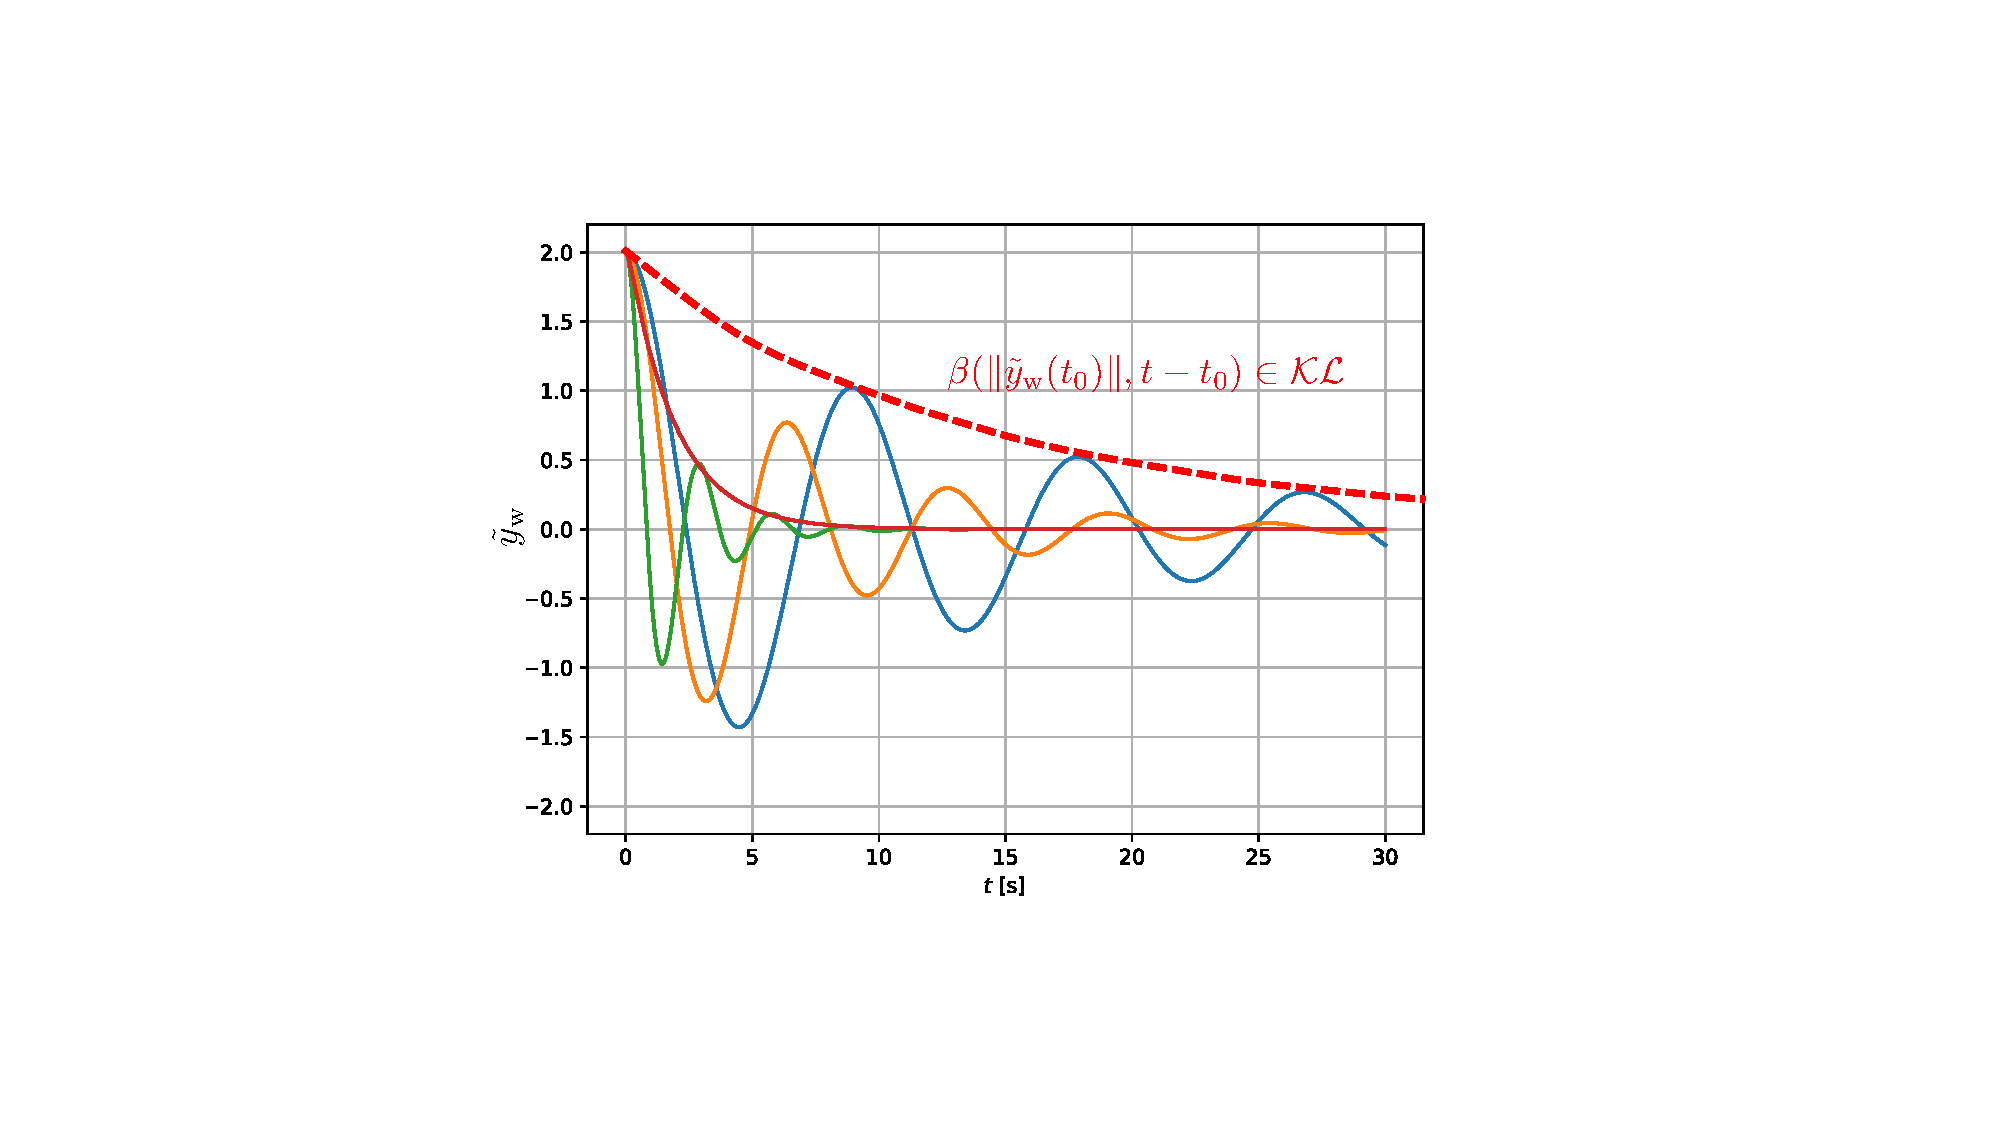
\includegraphics[width=0.46\columnwidth]{con/figures/iss/gas_illustration_cropped.pdf}}
    \subfigure[ISS]{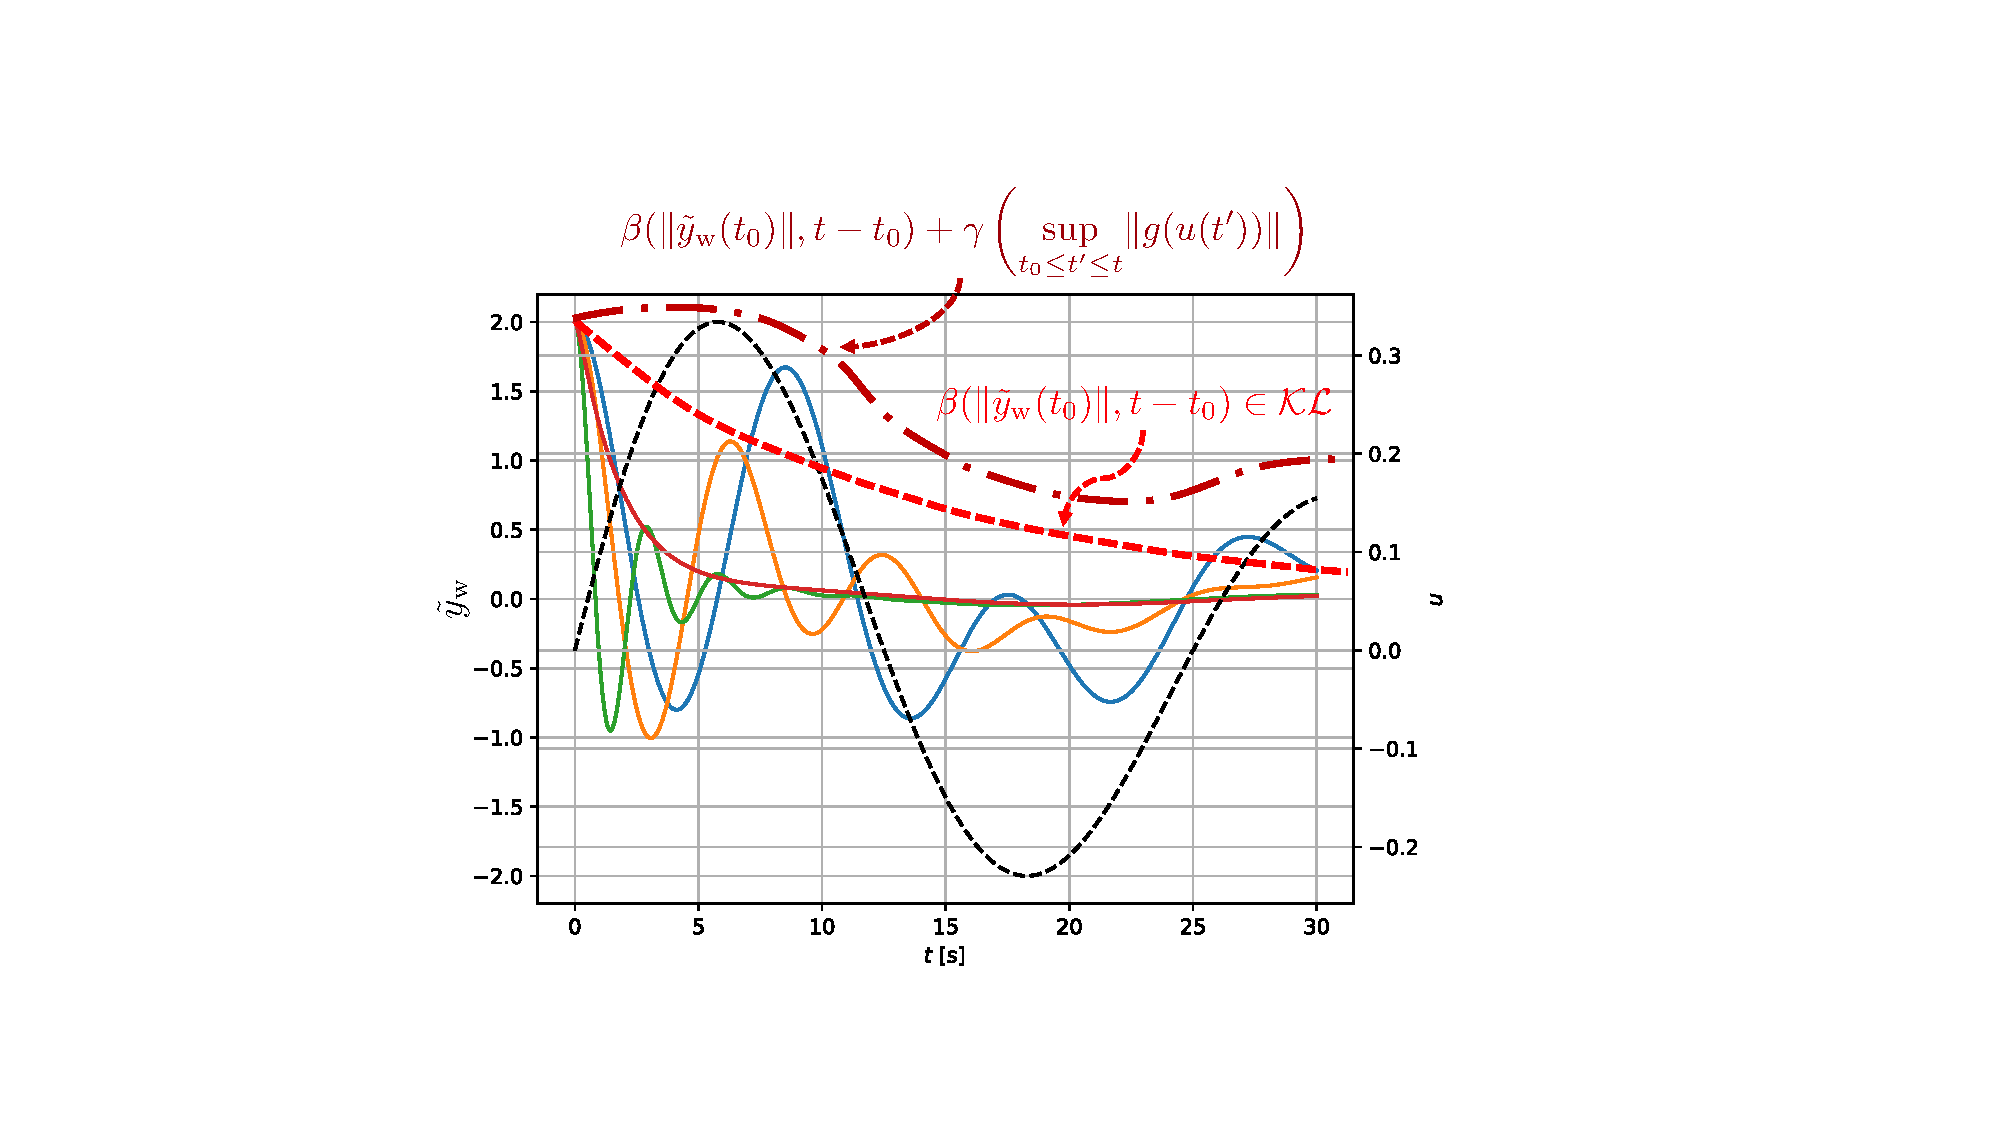
\includegraphics[width=0.49\columnwidth]{con/figures/iss/iss_illustration_cropped.pdf}}
    \caption{Illustration of global asymptotic stability for the unforced system with $g(u)=0$ and input-to-state stability for the forced system, where the black dashed line denotes the input $u(t)$.}
    \label{fig:con:gas_iss_illustration}
\end{figure}

\subsection{Global Asymptotic Stability (GAS) for the unforced system} 
We first consider the unforced system with $\tau = g(u) = 0, \: \forall t \in [t_0, t_\infty)$ and strive to prove global asymptotic stability~\cite{khalil2002nonlinear} for the attractor $\bar{x}$.
For this, we need to first identify a valid, (strict) Lyapunov function and subsequently demonstrate that, expect at the global equilibrium, the time derivative of the Lypapunov function is negative definite.

\subsubsection{Strict Lyapunov candidate}
We propose a strict Lyapunov candidate with skewed level sets~\cite{wu2022passive}
\begin{equation}\label{eq:con:conw_lyapunov_function}
\begin{split}
    V_\mu(\tilde{y}_\mathrm{w}) =& \: \frac{1}{2} \, \tilde{y}_\mathrm{w}^\mathrm{T} \, P_\mathrm{V} \, \tilde{y}_\mathrm{w} + \sum_{i=1}^n \int_{0}^{\tilde{x}_{\mathrm{w},i}} \tanh(\bar{x}_{\mathrm{w},i}+\sigma+b_i) \, \mathrm{d} \sigma - \sum_{i=1}^n \int_{0}^{\tilde{x}_{\mathrm{w},i}} \tanh(\bar{x}_{\mathrm{w},i}+b_i) \, \mathrm{d} \sigma,\\
    =& \: \frac{1}{2} \, \tilde{y}_\mathrm{w}^\mathrm{T} \, P_\mathrm{V} \, \tilde{y}_\mathrm{w} + \sum_{i=1}^n \left ( \mathrm{lcosh}(\bar{x}_{\mathrm{w},i} + \tilde{x}_{\mathrm{w},i}+b_i)-\mathrm{lcosh}(\bar{x}_{\mathrm{w},i}+b_i)-\tanh(\bar{x}_{\mathrm{w},i}+b_i) \, \tilde{x}_{\mathrm{w},i} \right ),\\
    \text{with } P_\mathrm{V} =& \: \begin{bmatrix}
        K_\mathrm{w} & \mu \, M_\mathrm{w}\\
        \mu \, M_\mathrm{w}^\mathrm{T} & M_\mathrm{w}
    \end{bmatrix} \in \mathbb{R}^{2n \times 2n}, \qquad \mathrm{lcosh}(\cdot) = \log(\cosh(\cdot)), \qquad \text{and } \mu > 0.
\end{split}
\end{equation}

In the following, we will write $\lVert A \rVert$ to denote the induced norm of matrix $A$ and $\lambda_\mathrm{m}(A)$, $\lambda_\mathrm{M}(A)$ to refer to its minimum and maximum Eigenvalue respectively.
% 
The gradient of $V_\mu(\tilde{y}_\mathrm{w})$ w.r.t. the residual coordinate $\tilde{y}_\mathrm{w}$ is given by
\begin{equation}\label{eq:con:V_mu_gradient}
    \frac{\partial V_\mu}{\partial \tilde{y}_\mathrm{w}}(\tilde{y}_\mathrm{w}) = P_\mathrm{V} \, \tilde{y}_\mathrm{w} + 
    \begin{bmatrix}
        \tanh(\bar{x}_\mathrm{w} + \tilde{x}_\mathrm{w} + b)\\ 
        0^{n}
    \end{bmatrix} - \begin{bmatrix}
        \tanh(\bar{x}_\mathrm{w} + b)\\ 
        0^{n}
    \end{bmatrix}.
\end{equation}
Next, the Hessian of the Lyapunov candidate can be derived as
\begin{equation}\label{eq:con:V_mu_hessian}
    H_\mathrm{V}(\tilde{x}_\mathrm{w}) = \frac{\partial^2 V_\mu}{\partial \tilde{y}_\mathrm{w}^2} = \begin{bmatrix}
        K_\mathrm{w} + S_\mathrm{sech}^{2}(\tilde{x}_\mathrm{w}) & \mu \, M_\mathrm{w}\\
        \mu \, M_\mathrm{w}^\mathrm{T} & M_\mathrm{w}
    \end{bmatrix} \in \mathbb{R}^{2n \times 2n},
\end{equation}
where
\begin{equation}\label{eq:con:S_sech_definition}
    S_\mathrm{sech}(\tilde{x}_\mathrm{w}) = \mathrm{diag}(\mathrm{sech}(\bar{x}_\mathrm{w} + \tilde{x}_\mathrm{w} + b)) \in \mathbb{R}^{n \times n} \succ 0 \quad \forall \tilde{x}_\mathrm{w} \in \mathbb{R}^n.
\end{equation}
Furthermore, the Schur complement of $P_\mathrm{V}$ is given by
\begin{equation}\label{eq:con:P_V_Schur_complement}
    S_{P_\mathrm{V}} = M_\mathrm{w} - \mu^2 M_\mathrm{w}^\mathrm{T} \, K_\mathrm{w} \, M_\mathrm{w}
\end{equation}

Below, we will first introduce three auxiliary Lemmas and subsequently proof Lemma~\ref{lemma:con:conw_lyapunov_candidate} that states that \eqref{eq:con:conw_lyapunov_function} is a valid Lyapunov candidate.

\begin{lemma}\label{lemma:con:P_V_Schur_complement_positive_definite}
    % Given $M_\mathrm{w} \succ 0, K_\mathrm{w} \succ 0$, we can always choose a positive constant $\mu > 0$ in \eqref{eq:con:conw_lyapunov_function} such that $S_\mathrm{w}(\tilde{y}_\mathrm{w})$ is positive definite.
    Suppose $M_\mathrm{w} \succ 0, K_\mathrm{w} \succ 0$ and $0 < \mu < \frac{\sqrt{\lambda_\mathrm{m}(M_\mathrm{w}) \, \lambda_\mathrm{m}\left(K_\mathrm{w}\right)}}{\lVert M_\mathrm{w} \rVert} \coloneqq \mu_\mathrm{V}$. Then $S_{P_\mathrm{V}}$, as defined in \eqref{eq:con:P_V_Schur_complement}, is positive definite.
\end{lemma}
\begin{proof}
    The minimum Eigenvalue of $S_{P_\mathrm{V}}$ is bounded by
    \begin{equation}
    \begin{split}
        \lambda_\mathrm{m}(S_{P_\mathrm{V}}) \geq& \: \lambda_\mathrm{m}(M_\mathrm{w}) - \mu^2 \, \lVert M_\mathrm{w}^\mathrm{T} \, K_\mathrm{w} \, M_\mathrm{w} \rVert,\\
        \geq& \: \lambda_\mathrm{m}(M_\mathrm{w}) - \mu^2 \, \frac{\lVert M_\mathrm{w} \rVert^2}{\lambda_\mathrm{w} \left (K_\mathrm{w} \right )}\\
    \end{split}
    \end{equation}
    Based on the assumption $M_\mathrm{w} \succ 0, K_\mathrm{w} \succ 0$, we can state $\frac{\lVert M_\mathrm{w} \rVert}{\lambda_\mathrm{w}(K_\mathrm{w})} > 0$. Therefore, the critical case for the lower bound on $\lambda_\mathrm{m}(S_{P_\mathrm{V}})$ is $
    \mu = \frac{\sqrt{\lambda_\mathrm{m}(M_\mathrm{w}) \, \lambda_\mathrm{m}\left(K_\mathrm{w}\right)}}{\lVert M_\mathrm{w} \rVert} \coloneqq \mu_\mathrm{V}$. Hence,
    \begin{equation}
    \begin{split}
        \lambda_\mathrm{m}(S_{P_\mathrm{V}}) >& \: \lambda_\mathrm{m}(M_\mathrm{w}) - \frac{\lambda_\mathrm{m}(M_\mathrm{w}) \, \lambda_\mathrm{m}\left(K_\mathrm{w}\right)}{\lVert M_\mathrm{w} \rVert^2} \, \frac{\lVert M_\mathrm{w} \rVert^2}{\lambda_\mathrm{w}(K_\mathrm{w})} \: = \: 0
    \end{split}
    \end{equation}
    Consequently, the Eigenvalue sensitivity theorem~\cite{golub2013matrix} demands that $S_{P_\mathrm{V}} \succ 0$.
\end{proof}

\begin{lemma}\label{lemma:con:P_V_positive_definite}
    Let $M_\mathrm{w} \succ 0, K_\mathrm{w} \succ 0$, and $0 < \mu < \frac{\sqrt{\lambda_\mathrm{m}(M_\mathrm{w}) \, \lambda_\mathrm{m}\left(K_\mathrm{w}\right)}}{\lVert M_\mathrm{w} \rVert} \coloneqq \mu_\mathrm{V}$. Then, it follows that $P_\mathrm{V} \succ 0$ and $H_\mathrm{V}(\tilde{x}_\mathrm{w}) \succ 0 \: \: \forall \: \tilde{x}_\mathrm{w}\in \mathbb{R}^n$.
\end{lemma}
\begin{proof}
    By inspecting the expressions for $P_\mathrm{V} \succ 0$ and $H_\mathrm{V}(\tilde{x}_\mathrm{w}) \succ 0 \: \forall \tilde{x}_\mathrm{w}\in \mathbb{R}^n$ in Equations \eqref{eq:con:conw_lyapunov_function} and \eqref{eq:con:V_mu_hessian}, respectively, it can be easily seen that $H_\mathrm{V}(\tilde{x}_\mathrm{w}) \succeq P_\mathrm{V} \: \forall \tilde{x}_\mathrm{w}\in \mathbb{R}$. As Lemma~\ref{lemma:con:P_V_Schur_complement_positive_definite} states that the Schur complement of $P_\mathrm{V}$ is positive definite, it follows that $H_\mathrm{V}(\tilde{x}_\mathrm{w}) \succeq P_\mathrm{V} \succ 0$.
\end{proof}

\begin{lemma}\label{lemma:con:V_tanh_term_lower_term}
    % The scalar function $h_\mathrm{V,th}(r) = \int_{0}^r \tanh(\sigma + a) \, \mathrm{d}\sigma - \int_{0}^r \tanh(a) \, \mathrm{d}\sigma$ with $r \in \mathbb{R}$ is positive semi-definite: $h_\mathrm{V,th}(r) \geq 0 \: \forall r \in \mathbb{R}$. 
    Suppose $\bar{x}_{\mathrm{w}}, \tilde{x}_{\mathrm{w}}, b \in \mathbb{R}^n$ and $n \in \mathbb{N}^+$. Then,
    \begin{equation}
        h_{\mathrm{V,th}}(\tilde{x}_{\mathrm{w}}) = \sum_{i=1}^n \int_{0}^{\tilde{x}_{\mathrm{w},i}} \tanh(\bar{x}_{\mathrm{w},i}+\sigma+b_i) \, \mathrm{d} \sigma - \sum_{i=1}^n \int_{0}^{\tilde{x}_{\mathrm{w},i}} \tanh(\bar{x}_{\mathrm{w},i}+b_i) \, \mathrm{d} \sigma
    \end{equation}
    is a positive semi-definite function.
\end{lemma}
\begin{proof}
    % $h_\mathrm{V,th}(r)$ can be rewritten as
    % \begin{equation}
    %     h_\mathrm{V,th}(r) = \log(\cosh(r+a))-\log(\cosh(a))-\tanh(a) \, r.
    % \end{equation}
    Proving $h_{\mathrm{V},\mathrm{th}}(\tilde{x}_\mathrm{w}) \geq 0$ is equivalent to showing that the scalar function $\breve{h}_{\mathrm{V},\mathrm{th}}(r) = \int_{0}^r \tanh(\sigma + a) \, \mathrm{d}\sigma - \int_{0}^r \tanh(a) \, \mathrm{d}\sigma \geq 0 \: \: \forall \: r, a \in \mathbb{R}$, where we set $r = \tilde{x}_{\mathrm{w},i}$ and $a = \bar{x}_{\mathrm{w},i} + b_i$.
    
    We strive to find the critical points (i.e., minimas and maximas) $\bar{r}$ of $\breve{h}_\mathrm{V,th}(r)$ and, for this, analyze where the first derivative of $\breve{h}_\mathrm{V,th}(r)$ is zero
    \begin{equation}
        \frac{\partial \breve{h}_\mathrm{V,th}}{\partial r}(\bar{r}) = \tanh(\bar{r}+a) - \tanh(a) = 0,
    \end{equation}
    which is the case only for $\bar{r}=0$. Next, we compute the second derivative at $\bar{r}$ as
    \begin{equation}
        \frac{\partial \breve{h}_\mathrm{V,th}}{\partial r}(\bar{r}) = \mathrm{sech}^2(\bar{r}) = 1.
    \end{equation}
    Thus, $\breve{h}_\mathrm{V,th}(r)$ is convex and its global minimum at $\bar{r}=0$ takes the value $h_\mathrm{V,th}(0) = 0$.
    As a result, $h_{\mathrm{V},\mathrm{th}}(\tilde{x}_\mathrm{w})$ is also positive semi-definite.
\end{proof}

\begin{lemma}\label{lemma:con:conw_lyapunov_candidate}
    The scalar function $V_\mu(\tilde{y}_\mathrm{w})$ defined in \eqref{eq:con:conw_lyapunov_function} is continuously differentiable and verifies the condition $V_\mu(0) = 0$.
    Furthermore, let $M_\mathrm{w}, K_\mathrm{w} \succ 0$.
    Now, if we choose $0 < \mu < \frac{\sqrt{\lambda_\mathrm{m}(M_\mathrm{w}) \, \lambda_\mathrm{m}\left(K_\mathrm{w}\right)}}{\lVert M_\mathrm{w} \rVert} \coloneqq \mu_\mathrm{V}$, then $V_\mu(\tilde{y}_\mathrm{w}) > 0 \: \forall \: \tilde{y}_\mathrm{w} \in \mathbb{R}^{2n} \setminus \{0 \}$. Additionally, then $V_\mu(\tilde{y}_\mathrm{w})$ is radially unbounded as $\lVert \tilde{y}_\mathrm{w} \rVert \rightarrow \infty \Rightarrow V_\mu(\tilde{y}_\mathrm{w}) \rightarrow \infty$.
    % ($V_\mu(\tilde{y}_\mathrm{w})$ is globally positive definite)
    % ($V_\mu(\tilde{y}_\mathrm{w})$ is radially unbounded)
\end{lemma}
\begin{proof}

    \textbf{Step 1:} 
    % Proof that the Lyapunov candidate is continuously differentiable. 
    It can be easily seen that $V_\mu(\tilde{y}_\mathrm{w})$ in \eqref{eq:con:conw_lyapunov_function} is smooth and continuously differentiable.
    
    \textbf{Step 2:} Proof that $V_\mu(0) = 0$.
    \begin{equation}
        V_\mu(0) = 0 + \sum_{i=1}^n \int_{0}^{0} \tanh(\bar{y}_{\mathrm{w},i}+\sigma+b_i) \, \mathrm{d} \sigma - \sum_{i=1}^n \int_{0}^{0} \tanh(\bar{y}_{\mathrm{w},i}+b_i) \, \mathrm{d} \sigma = 0.
    \end{equation}
    
    \textbf{Step 3:} Proof that the Lyapunov candidate is positive definite; i.e., $V_\mu(\tilde{y}_\mathrm{w}) > 0 \: \: \forall \tilde{y}_\mathrm{w} \in \mathbb{R}^n \setminus \{0 \}$.
    % If we can show that $V_\mu(\tilde{y}_\mathrm{w})$ is convex with the global minimum at $\tilde{y}_\mathrm{w} = 0$, we will have demonstrated this characteristic to be true.
    
    As the gradient of the Lyapunov candidate, as defined in \eqref{eq:con:V_mu_gradient}, is zero for $\tilde{y}_\mathrm{w} = 0$: \begin{equation}
        \frac{\partial V_\mu}{\partial \tilde{y}_\mathrm{w}}(0) = \begin{bmatrix}
            \tanh(\bar{x}_\mathrm{w} + b)\\ 
            0^{n}
        \end{bmatrix} - \begin{bmatrix}
            \tanh(\bar{x}_\mathrm{w} + b)\\ 
            0^{n}
        \end{bmatrix} = 0,
    \end{equation}
    $\tilde{y}_\mathrm{w} = 0$ is a critical point of $V_\mu(\tilde{y}_\mathrm{w})$. 
    According to Lemma~\ref{lemma:con:P_V_positive_definite}, the Hessian in \eqref{eq:con:V_mu_hessian} is positive-definite~\cite{boyd2004convex}: $H_\mathrm{V}(\tilde{y}_\mathrm{w}) \succ 0 \: \: \forall \tilde{y}_\mathrm{w} \in \mathbb{R}^{2n}$.
    With that, \eqref{eq:con:conw_lyapunov_function} is convex and its global minimum is at $\tilde{y}_\mathrm{w} = 0$, where $V_\mu(0) = 0$. In summary, we state $V_\mu(\tilde{y}_\mathrm{w}) > 0 \: \: \forall \tilde{y}_\mathrm{w} \in \mathbb{R}^n \setminus \{0 \}$.

    \textbf{Step 4:} Proof that the Lyapunov candidate is radially unbounded: i.e., $\lVert \tilde{y}_\mathrm{w} \rVert \rightarrow \infty \Rightarrow V_\mu(\tilde{y}_\mathrm{w}) \rightarrow \infty$. Lemma~\ref{lemma:con:V_tanh_term_lower_term} is exploited for identifying a lower bound on $V_\mu(\tilde{y}_\mathrm{w})$:
    \begin{equation}
    \begin{split}
        V_\mu(\tilde{y}_\mathrm{w}) =& \: \frac{1}{2} \, \tilde{y}_\mathrm{w}^\mathrm{T} \, P_\mathrm{V} \, \tilde{y}_\mathrm{w} + \sum_{i=1}^n \int_{0}^{\tilde{x}_{\mathrm{w},i}} \tanh(\bar{x}_{\mathrm{w},i}+\sigma+b_i) \, \mathrm{d} \sigma - \sum_{i=1}^n \int_{0}^{\tilde{x}_{\mathrm{w},i}} \tanh(\bar{x}_{\mathrm{w},i}+b_i) \, \mathrm{d} \sigma,\\
        % =& \: \frac{1}{2} \, \tilde{y}_\mathrm{w}^\mathrm{T} \, P_\mathrm{V} \, \tilde{y}_\mathrm{w} + \sum_{i=1}^n h_\mathrm{V,th,i}(\tilde{x}_{\mathrm{w}, i}), \qquad \text{with } a_i = \bar{y}_{\mathrm{w},i} + b_i,\\
        \geq& \: \frac{1}{2} \, \tilde{y}_\mathrm{w}^\mathrm{T} \, P_\mathrm{V} \, \tilde{y}_\mathrm{w} \: \geq \: \frac{1}{2} \, \lambda_\mathrm{m}(P_\mathrm{V}) \, \lVert \tilde{y}_\mathrm{w} \rVert^2.
    \end{split}
    \end{equation}
    Lemma~\ref{lemma:con:P_V_positive_definite} tells us that $P_\mathrm{V} \succ 0$ and with that $\lambda_\mathrm{m}(P_\mathrm{V}) > 0$. Therefore, if $\lVert \tilde{y}_\mathrm{w} \rVert \rightarrow \infty$, it also follows that $V_\mu(\tilde{y}_\mathrm{w}) \rightarrow \infty$.
\end{proof}

\subsubsection{Proof of global asymptotic stability}

In the following, we will demonstrate how the strict Lyapunov candidate of \eqref{eq:con:conw_lyapunov_function} allows us to prove global asymptotic stability of the unforced system. We will first introduce two auxiliary Lemmas before stating Theorem~\ref{theorem:con:global_asymptotic_stability}.

\begin{lemma}\label{lemma:con:V_d_tanh_term_lower_bound}
    Suppose $\bar{x}_\mathrm{w}, \tilde{x}_\mathrm{w}, b \in \mathbb{R}^n$ and $n \in \mathbb{N}^+$. Then, the function $h_{\dot{\mathrm{V}},\mathrm{th}}(\tilde{x}_\mathrm{w})$ defined as
    \begin{equation}
        h_{\dot{\mathrm{V}},\mathrm{th}}(\tilde{x}_\mathrm{w}) = \left ( \tanh(\bar{x}_\mathrm{w} + \tilde{x}_\mathrm{w} + b) - \tanh(\bar{x}_\mathrm{w} + b) \right )^\mathrm{T} \, \tilde{x}_\mathrm{w},
    \end{equation}
    is positive semi-definite.
\end{lemma}
\begin{proof}
    Proving $h_{\dot{\mathrm{V}},\mathrm{th}}(\tilde{x}_\mathrm{w}) \geq 0$ is equivalent to proving that the scalar function $\breve{h}_{\dot{\mathrm{V}},\mathrm{th}}(r) = \left ( \tanh(r + a) - \tanh(a) \right ) \, r \geq 0 \: \: \forall \: r, a \in \mathbb{R}$, where we set $r = \tilde{x}_{\mathrm{w},i}$ and $a = \bar{x}_{\mathrm{w},i} + b_i$.
    Now, we expand the hyperbolic tangent:
    \begin{equation}
    \begin{split}
        \breve{h}_{\dot{\mathrm{V}},\mathrm{th}}(r) =& \: \left ( \tanh(r + a) - \tanh(a) \right ) \, r = \left ( \frac{e^{2(r+a)}-1}{e^{2(r+a)}+1} - \frac{e^{2a}-1}{e^{2a}+1} \right ) \, r,\\
        =& \: \frac{2 \, e^{2a} \, \left ( e^{2r} - 1 \right )}{e^{2r+4a}+e^{2r + 2a}+e^{2a}+1} r \, \geq 0,
    \end{split}
    \end{equation}
    as the denominator $e^{2r+4a}+e^{2r + 2a}+e^{2a}+1 > 0 \:\: \forall \: r \in \mathbb{R}$ and as $\mathrm{sign} \left (2 \, e^{2a} \, \left ( e^{2r} - 1 \right ) \right) = \mathrm{sign}(r)$. For example, $e^{2r} - 1 \geq 0 \: \forall \: r \geq 0$. Analog, $e^{2r} - 1 < 0 \: \forall \: r < 0$. 
\end{proof}

\begin{lemma}\label{lemma:con:P_V_d_positive_definite}
    Let $M_\mathrm{w} \succ 0$, $K_\mathrm{w} \succ 0$, and $D_\mathrm{w} \succ 0$. Also, let $\mu \in \mathbb{R}^+$ be chosen such that $0 < \mu < \frac{\lambda_\mathrm{m}(D_\mathrm{w})}{\lambda_\mathrm{m}(M_\mathrm{w}) + \frac{\lVert D_\mathrm{w} \rVert^2}{4 \lambda_\mathrm{m} (K_\mathrm{w})}} \coloneqq \mu_{\dot{\mathrm{V}}}$.
    Then, the matrix $P_{\dot{V}} = \begin{bmatrix}
        \mu K_\mathrm{w} & \frac{1}{2} \mu D_\mathrm{w}\\
        \frac{1}{2} \mu D_\mathrm{w}^\mathrm{T} & D_\mathrm{w} - \mu M_\mathrm{w}
    \end{bmatrix} \in \mathbb{R}^{n}$ is positive definite.
\end{lemma}
\begin{proof}
    The Schur complement of $P_{\dot{V}}$ is given by
    \begin{equation}
        S_{P_{\dot{V}}} = D_\mathrm{w} - \mu M_\mathrm{w} - \frac{1}{4} \, \mu D_\mathrm{w}^\mathrm{T} \, K_\mathrm{w}^{-1} \, D_\mathrm{w}.
    \end{equation}
    The lower bound on the smallest Eigenvalue of $S_{P_{\dot{V}}}$ can be identified as
    \begin{equation}
        \lambda_\mathrm{m} \left (S_{P_{\dot{V}}} \right ) \geq \lambda_\mathrm{m}(D_\mathrm{w}) - \mu \, \lambda_\mathrm{m}(M_\mathrm{w}) - \mu \frac{\lVert D_\mathrm{w} \rVert^2}{4 \, \lambda_\mathrm{m}(K_\mathrm{w})}.
    \end{equation}
    As $K_\mathrm{w}, D_\mathrm{w} \succ 0$, we know that $\frac{\lVert D_\mathrm{w} \rVert^2}{\lambda_\mathrm{m}(K_\mathrm{w})} > 0$. Therefore, the case $\mu = \frac{\lambda_\mathrm{m}(D_\mathrm{w})}{\lambda_\mathrm{m}(M_\mathrm{w}) + \frac{\lVert D_\mathrm{w} \rVert^2}{4 \lambda_\mathrm{m} (K_\mathrm{w})}} \coloneqq \mu_{\dot{\mathrm{V}}}$ determines the lower bound on $\lambda_\mathrm{m}(S_{P_{\dot{V}}})$:
    \begin{equation}
    \begin{split}
        \lambda_\mathrm{m} \left (S_{P_{\dot{V}}} \right ) > \lambda_\mathrm{m}(D_\mathrm{w}) - \mu_{\dot{\mathrm{V}}} \left ( \lambda_\mathrm{m}(M_\mathrm{w}) - \frac{\lVert D_\mathrm{w} \rVert^2}{4 \, \lambda_\mathrm{m}(K_\mathrm{w})} \right ) = 0.
    \end{split}
    \end{equation}
    We conclude, based on the Eigenvalue sensitivity theorem of symmetric matrices~\cite{golub2013matrix}, that $S_{P_{\dot{V}}} \succ 0$ and with that $P_{\dot{V}} \succ 0$~\cite{boyd2004convex}.
\end{proof}

\begin{theorem}\label{theorem:con:global_asymptotic_stability}
    Let $M_\mathrm{w}, K_\mathrm{w}$ and $D_\mathrm{w}$ be positive definite and suppose the system be unforced: $g(u(t)) = 0$.
    Then, $\tilde{y}_\mathrm{w} = 0$ is globally asymptotically stable for the system dynamics defined \eqref{eq:con:conw_residual_dynamics} such that $\dot{V}_\mu (\tilde{y}_\mathrm{w}) < 0, \quad \forall \: \tilde{y}_\mathrm{w} \in \mathbb{R}^{2n} \setminus \{0 \}$.
    
    % around the equilibrium $\tilde{y}_\mathrm{w} = 0$ if $g(u(t)) = 0$, $M_\mathrm{w} \succ 0$, $K_\mathrm{w} \succ 0$, and $D_\mathrm{w} \succ 0$.
\end{theorem}
\begin{proof}
    First, we show that $\tilde{y}_\mathrm{w} = 0$ is an equilibrium of \eqref{eq:con:conw_residual_dynamics}:
    \begin{equation}
        \tilde{f}_\mathrm{w}(0, 0) = \begin{bmatrix}
            0\\
            M_\mathrm{w}^{-1} \, \left (-K_\mathrm{w} \, \bar{x}_\mathrm{w} - \tanh(\bar{x}_\mathrm{w} + b) \right )
        \end{bmatrix}
        = \begin{bmatrix}
            0\\
            M_\mathrm{w}^{-1} \, \left (-K_\mathrm{w} \, \bar{x}_\mathrm{w} + K_\mathrm{w} \, \bar{x}_\mathrm{w} \right )
        \end{bmatrix}
        = \begin{bmatrix}
            0\\
            0
        \end{bmatrix}
    \end{equation}

    Lemma~\ref{lemma:con:conw_lyapunov_candidate} states that we can always choose $\mu$ such that \eqref{eq:con:conw_lyapunov_function} is strict Lyapunov function (e.g., Lipschitz continuous, zero-valued at $\tilde{y}_\mathrm{w} = 0$, positive definite, and radially unbounded)~\cite{khalil2002nonlinear, wu2022passive}. We now evaluate the time-derivative of $\dot{V}_\mu(\tilde{y}_\mathrm{w})$ in the case of an unforced system (i.e., $g(u(t)) = 0$):
    \begin{equation}\label{eq:con:lyapunov_function_time_derivative}
    \begin{split}
        \dot{V}_\mu(\tilde{y}_\mathrm{w}) =& \: \frac{\partial V_\mu}{\partial \tilde{y}_\mathrm{w}} \, \dot{\tilde{y}}_\mathrm{w} = \frac{\partial V_\mu}{\partial \tilde{y}_\mathrm{w}} \, \tilde{f}_\mathrm{w}(\tilde{y}_\mathrm{w}) 
        % = \frac{\partial \dot{V}_\mu}{\partial \tilde{x}_\mathrm{w}} \, \tilde{\dot{x}}_\mathrm{w} + \frac{\partial \dot{V}_\mu}{\partial \tilde{\dot{x}}_\mathrm{w}} \, \tilde{f}_{\mathrm{w}, \ddot{\tilde{x}}_\mathrm{w}}(\tilde{y}_\mathrm{w}) 
        = \tilde{y}_\mathrm{w}^\mathrm{T} \, P_\mathrm{V} \, \dot{\tilde{y}}_\mathrm{w} + \left (\tanh(\bar{x}_\mathrm{w} + \tilde{x}_\mathrm{w} + b) - \tanh(\bar{x}_\mathrm{w} + b)\right )^\mathrm{T} \, \dot{\tilde{x}}_\mathrm{w}\\
        =& \: -\tilde{y}_\mathrm{w}^\mathrm{T} \, \underbrace{\begin{bmatrix}
            \mu \, K_\mathrm{w} & \frac{1}{2} \, \mu \, D_\mathrm{w}\\
            \frac{1}{2} \, \mu \, D_\mathrm{w}^\mathrm{T} & D_\mathrm{w} - \mu \, M_\mathrm{w}
        \end{bmatrix}}_{P_{\dot{\mathrm{V}}}} \, \tilde{y}_\mathrm{w} - \mu \left ( \tanh(\bar{x}_\mathrm{w} + \tilde{x}_\mathrm{w} + b)^\mathrm{T} + \tilde{x}_\mathrm{w}^\mathrm{T} \, K_\mathrm{w} \right ) \tilde{x}_\mathrm{w},\\
        =& \: -\tilde{y}_\mathrm{w}^\mathrm{T} \, P_{\dot{\mathrm{V}}} \, \tilde{y}_\mathrm{w} - \mu \, \left ( \tanh(\bar{x}_\mathrm{w} + \tilde{x}_\mathrm{w} + b) - \tanh(\bar{x}_\mathrm{w} + b) \right )^\mathrm{T} \tilde{x}_\mathrm{w},\\
        \leq& \: -\tilde{y}_\mathrm{w}^\mathrm{T} \, P_{\dot{\mathrm{V}}} \, \tilde{y}_\mathrm{w} 
        \: \leq \: -\lambda_\mathrm{m}\left(P_{\dot{\mathrm{V}}} \right) \, \lVert \tilde{y}_\mathrm{w} \rVert_2^2,
    \end{split}
    \end{equation}
    where we exploited the force balance at equilibrium $K_\mathrm{w} \, \bar{x}_\mathrm{w} = -\tanh(\bar{x}_\mathrm{w} + b)$ and Lemma~\ref{lemma:con:V_d_tanh_term_lower_bound} for defining the upper bound on $\dot{V}_\mu(\tilde{y}_\mathrm{w})$. Lemma~\ref{lemma:con:P_V_d_positive_definite} states that $P_{\dot{\mathrm{V}}} \succ 0$ for $0 < \mu < \mu_{\dot{\mathrm{V}}}$. Similarly, Lemma~\ref{lemma:con:conw_lyapunov_candidate} requests that $0 < \mu < \mu_{\mathrm{V}}$. Indeed, both conditions can always be fulfilled by choosing $\mu \in \left (0, \min \{ \mu_{\mathrm{V}}, \mu_{\dot{\mathrm{V}}} \} \right )$. 
    With $P_{\dot{\mathrm{V}}} \succ 0 \Leftrightarrow \lambda_\mathrm{m}\left(P_{\dot{\mathrm{V}}} \right) > 0$~\cite{golub2013matrix}, we can state that $\dot{V}_\mu(\tilde{y}_\mathrm{w}) < 0 \: \forall \: \tilde{y}_\mathrm{w} \in \mathbb{R}^{2n} \setminus \{0 \}$ and conclude that the unforced system is globally asymptotically stable around $\tilde{y}_\mathrm{w} = 0$.
\end{proof}

\subsection{Global Input-to-State Stability (ISS) for the forced system} 
We now take the forcing $g(u)$ into account again and demonstrate that the system states remain proportionally bounded to the initial conditions and as a function of the supremum of the input forcing.
In the following, we will first state two auxiliary Lemmas and subsequently prove Theorem~\ref{theorem:con:iss} to provides the conditions for \gls{ISS}.

\begin{lemma}\label{lemma:con:V_tanh_term_upper_bound}
    Let $\bar{x}_{\mathrm{w}}, \tilde{x}_{\mathrm{w}}, b \in \mathbb{R}^n$.
    Then,
    \begin{equation}
        h_{\mathrm{V},th}(\tilde{x}_{\mathrm{w}}) = \sum_{i=1}^n \int_{0}^{\tilde{x}_{\mathrm{w},i}} \tanh(\bar{x}_{\mathrm{w},i}+\sigma+b_i) \, \mathrm{d} \sigma - \sum_{i=1}^n \int_{0}^{\tilde{x}_{\mathrm{w},i}} \tanh(\bar{x}_{\mathrm{w},i}+b_i) \, \mathrm{d} \sigma \leq 2 \, \left | \tilde{x}_{\mathrm{w}} \right |.
    \end{equation}
\end{lemma}
\begin{proof}
    Proving $h_{\mathrm{V},th}(\tilde{x}_{\mathrm{w}}) \leq 2 \, \left | \tilde{x}_{\mathrm{w}} \right |$ is equivalent to proving that the scalar function $\breve{h}_{\mathrm{V},\mathrm{th}}(r) = \int_0^{r} \tanh(\sigma + a) \: \mathrm{d}\sigma - \int_0^{r} \tanh(a) \: \mathrm{d}\sigma  \leq 2 \, |r| \: \: \forall \: r, a \in \mathbb{R}$, where we set $r = \tilde{x}_{\mathrm{w},i}$ and $a = \bar{x}_{\mathrm{w},i} + b_i$.
    We perform the integration contained in $\breve{h}_{\mathrm{V},\mathrm{th}}(r)$:
    \begin{equation}
    \begin{split}
        \breve{h}_{\mathrm{V},\mathrm{th}}(r) =& \: \int_0^{r} \tanh(\sigma + a) \: \mathrm{d}\sigma - \int_0^{r} \tanh(a) \: \mathrm{d}\sigma,\\
        \breve{h}_{\mathrm{V},\mathrm{th}}(r) =& \: \log(\cosh(r+a)) - \log(\cosh(a)) - \tanh(a) \, r.
    \end{split}
    \end{equation}
    Next, we demonstrate that the slope of $2 \, |r|$ is always larger than the magnitude of the slope of $\breve{h}_{\mathrm{V},\mathrm{th}}(r)$:
    \begin{equation}
    \begin{split}
        \left | \frac{\partial \breve{h}_{\mathrm{V},\mathrm{th}}}{\partial r} \right | =& \: \left | \tanh(r+a) - \tanh(a) \right | < 2 = \frac{\partial}{\partial r} \, (2 \, |r|).\\
    \end{split}
    \end{equation}
    Additionally, $\breve{h}_{\mathrm{V},\mathrm{th}}(0) = 2 \, |0| = 0$. We conclude that $\breve{h}_{\mathrm{V},\mathrm{th}}(r) \leq 2 |r| \: \forall \: r \in \mathbb{R}$ and with that, $h_{\mathrm{V},th}(\tilde{x}_{\mathrm{w}}) \leq 2 \, \left | \tilde{x}_{\mathrm{w}} \right | \: \forall \: \tilde{x}_{\mathrm{w}} \in \mathbb{R}^n$.
\end{proof}

\begin{lemma}\label{lemma:con:iss_lyapunov_bounds}
    % Assuming that $M_\mathrm{w} \succ 0$ and $K_\mathrm{w} \succ 0$, we can state that the 
    Let $M_\mathrm{w} \succ 0$ and $K_\mathrm{w} \succ 0$. Then, \eqref{eq:con:conw_lyapunov_function} is bounded by the two scalar, class $\mathcal{K}_\infty$ functions $\alpha_1(r)=\frac{1}{2} \, \lambda_\mathrm{m}(P_\mathrm{V})  \, r^2$ and $\alpha_2(r)=\frac{1}{2} \, \lambda_\mathrm{M}(P_\mathrm{V}) \, r^2 + 2 \, \sqrt{n} \, r$: $ \alpha_1(\lVert \tilde{y}_\mathrm{w} \rVert_2^2) \leq V_\mu(\tilde{y}_\mathrm{w}) \leq \alpha_2(\lVert \tilde{y}_\mathrm{w} \rVert)_2^2$.
\end{lemma}
\begin{proof}
    With Lemma~\ref{lemma:con:conw_lyapunov_candidate}, we already showed that  $V_\mu(\tilde{y}_\mathrm{w})$ is a Lyapunov candidate. Now, we additionally also verify the conditions for ISS-Lyapunov candidates~\cite{khalil2002nonlinear}.

    \textbf{Step 1:} Establishing bounds on $V_\mu(\tilde{y}_\mathrm{w})$.\\
    We first identify the lower bound of $V_\mu(\tilde{y}_\mathrm{w})$ by leveraging Lemma~\ref{lemma:con:V_tanh_term_lower_term}:
    \begin{equation}
    \begin{split}
        V_\mu(\tilde{y}_\mathrm{w}) =& \: \frac{1}{2} \, \tilde{y}_\mathrm{w}^\mathrm{T} \, P_\mathrm{V} \, \tilde{y}_\mathrm{w} + \sum_{i=1}^n \int_{0}^{\tilde{x}_{\mathrm{w},i}} \tanh(\bar{x}_{\mathrm{w},i}+\sigma+b_i) \, \mathrm{d} \sigma - \sum_{i=1}^n \int_{0}^{\tilde{x}_{\mathrm{w},i}} \tanh(\bar{x}_{\mathrm{w},i}+b_i) \, \mathrm{d} \sigma,\\
        =& \: \frac{1}{2} \, \tilde{y}_\mathrm{w}^\mathrm{T} \, P_\mathrm{V} \, \tilde{y}_\mathrm{w} + h_{\mathrm{V},\mathrm{th}}(\tilde{x}_\mathrm{w}),\\
        \geq& \: \frac{1}{2} \, \tilde{y}_\mathrm{w}^\mathrm{T} \, P_\mathrm{V} \, \tilde{y}_\mathrm{w}
        \: \geq \: \frac{1}{2} \, \lambda_\mathrm{m}(P_\mathrm{V}) \, \lVert \tilde{y}_\mathrm{w} \rVert_2^2
        \: = \: \alpha_1(\lVert \tilde{y}_\mathrm{w} \rVert_2).
    \end{split}
    \end{equation}
    Similarly, we derive an upper bound for $V_\mu(\tilde{y}_\mathrm{w})$ exploiting Lemma~\ref{lemma:con:V_tanh_term_upper_bound}.
    \begin{equation}
    \begin{split}
        V_\mu(\tilde{y}_\mathrm{w}) =& \frac{1}{2} \, \tilde{y}_\mathrm{w}^\mathrm{T} \, P_\mathrm{V} \, \tilde{y}_\mathrm{w} + \sum_{i=1}^n \int_{0}^{\tilde{x}_{\mathrm{w},i}} \tanh(\bar{x}_{\mathrm{w},i}+\sigma+b_i) \, \mathrm{d} \sigma - \sum_{i=1}^n \int_{0}^{\tilde{x}_{\mathrm{w},i}} \tanh(\bar{x}_{\mathrm{w},i}+b_i) \, \mathrm{d} \sigma\\
        \leq& \: \frac{1}{2} \, \lambda_\mathrm{M}(P_\mathrm{V}) \, \lVert \tilde{y}_\mathrm{w} \rVert_2^2 + 2 \, \lVert\tilde{x}_\mathrm{w}\rVert_1
        \: \leq \: \frac{1}{2} \, \lambda_\mathrm{M}(P_\mathrm{V}) \, \lVert \tilde{y}_\mathrm{w} \rVert_2^2 + 2 \, \sqrt{n} \, \lVert\tilde{x}_\mathrm{w}\rVert_2\\
        \leq& \: \frac{1}{2} \, \lambda_\mathrm{M}(P_\mathrm{V}) \, \lVert \tilde{y}_\mathrm{w} \rVert_2^2 + 2 \, \sqrt{n} \, \lVert\tilde{y}_\mathrm{w}\rVert_2 = \alpha_2(\lVert\tilde{y}_\mathrm{w}\rVert_2).
    \end{split}
    \end{equation}

    \textbf{Step 2:} Proof that $\alpha_1(r), \alpha_2(r)$ belong to class $\mathcal{K}_\infty$.\\
    According to Lemma~\ref{lemma:con:P_V_positive_definite}, $P_\mathrm{V} \succ 0$ and with that $\lambda_\mathrm{m}(P_\mathrm{V}) > 0$.
    First, we analyze the behavior of $\alpha_1(r)$: as it is strictly increasing and $\alpha_1(0) = 0$, it belongs to class $\mathcal{K}$. Furthermore, we can evaluate $\lim_{r \rightarrow \infty} \alpha_1(r) = \infty$. Therefore, $\alpha_1(r) \in \mathcal{K}_\infty$~\cite{khalil2002nonlinear}.
    $\alpha_2(r)$ is also strictly increasing for $r \in [0, \infty)$, $\alpha_2(0) = 0$, and it is radially unbounded as $\lim_{r \rightarrow \infty} \alpha_2(r) = \infty$. For that reason, $\alpha_2(r) \in \mathcal{K}_\infty$ as well.
\end{proof}

\begin{theorem}\label{theorem:con:iss}
    Suppose $M_\mathrm{w}, K_\mathrm{w}, D_\mathrm{w} \succ 0$, $0 < \theta < 1$, and that we choose $0 < \mu < \min \{ \mu_{\mathrm{V}}, \mu_{\dot{\mathrm{V}}} \}\}$. Then,
    \eqref{eq:con:conw_residual_dynamics} is globally Input-to-State Stable (ISS)
    such that the solution $\tilde{y}_\mathrm{w}(t)$ verifies
    \begin{equation}\label{eq:con:input_to_state_stability}
        \lVert \tilde{y}_\mathrm{w} \rVert_2 \leq \beta \left (\lVert \tilde{y}_\mathrm{w}(t_0) \rVert_2, t-t_0 \right ) + \gamma \left ( \sup_{t_0 \leq t' \leq t} \lVert g(u(t')) \rVert_2 \right ), \qquad \forall \: t \geq t_0
    \end{equation}
    where $\beta(r, t) \in \mathcal{KL}$, $\gamma(r) = \sqrt{\frac{(1+\mu^2) \, \lambda_\mathrm{M}(P_\mathrm{V}) \, r^2 + 4 \, \theta \, \sqrt{n} \, \sqrt{1+\mu^2} \, \lambda_\mathrm{m}(P_{\dot{\mathrm{V}}}) \, r}{\theta^2 \, \lambda_\mathrm{m}(P_\mathrm{V}) \, \lambda_\mathrm{m}^2(P_{\dot{\mathrm{V}}})}} \in \mathcal{K}$.
\end{theorem}
\begin{proof}

    % \textbf{Step 1:} Proof that $\gamma(r) \in \mathcal{K}$.
    % From Theorem~\ref{theorem:con:global_asymptotic_stability} and the associated proof, we know that $\lambda_\mathrm{m}(P_\mathrm{V}), \lambda_\mathrm{M}(P_\mathrm{V}), \lambda_\mathrm{m}(P_{\dot{\mathrm{V}})} > 0$ for suitable choices $0 < \mu < \min \{ \mu_\mathrm{V}, \mu_{\dot{\mathrm{V}}}$. Furthermore, we define $0 < \theta < 0$. 
    \textbf{Step 1:} Bounds on ISS-Lyapunov candidate.\\
    Lemma~\ref{lemma:con:iss_lyapunov_bounds} provides the $\mathcal{K_\infty}$ functions 
    $\alpha_1(r)=\frac{1}{2} \, \lambda_\mathrm{m}(P_\mathrm{V})  \, r^2$ and $\alpha_2(r)=\frac{1}{2} \, \lambda_\mathrm{M}(P_\mathrm{V}) \, r^2 + 2 \, \sqrt{n} \, r$ such that $ \alpha_1(\lVert \tilde{y}_\mathrm{w} \rVert_2^2) \leq V_\mu(\tilde{y}_\mathrm{w}) \leq \alpha_2(\lVert \tilde{y}_\mathrm{w} \rVert)_2^2$.
    % that represent the lower and upper bound on $V_\mu(\tilde{y}_\mathrm{w})$, respectively. 
    
    \textbf{Step 2:} Minimum energy dissipation.\\
    % For ISS, it is required that $\dot{V}_\mu(\tilde{y}_\mathrm{w}, u(t)) \leq -\alpha_3(\tilde{y}_\mathrm{w}), \quad \forall \: \lVert \tilde{y}_\mathrm{w} \rVert_2 \geq \rho$.\
    Let $0 < \mu < \min \{ \mu_{\mathrm{V}}, \mu_{\dot{\mathrm{V}}} \}\}$ as in the proof of Theorem~\ref{theorem:con:global_asymptotic_stability}.
    We compute the input-dependent time-derivative of the ISS Lyapunov candidate. We do not repeat the derivations already made as part of \eqref{eq:con:lyapunov_function_time_derivative} (e.g., exploiting Lemmas~\ref{lemma:con:V_d_tanh_term_lower_bound} and \ref{lemma:con:P_V_d_positive_definite}).
    \begin{equation}
    \begin{split}
        \dot{V}_\mu(\tilde{y}_\mathrm{w}, u(t)) =& \: % \frac{\partial V_\mu}{\partial \tilde{y}_\mathrm{w}} \, \tilde{f}_\mathrm{w}(\tilde{y}_\mathrm{w}, u(t)) = 
        -\tilde{y}_\mathrm{w}^\mathrm{T} \, P_{\dot{\mathrm{V}}} \, \tilde{y}_\mathrm{w} - \mu \, \left ( \tanh(\bar{x}_\mathrm{w} + \tilde{x}_\mathrm{w} + b) - \tanh(\bar{x}_\mathrm{w} + b) \right )^\mathrm{T} \tilde{x}_\mathrm{w} + \tilde{y}_\mathrm{w}^\mathrm{T} \begin{bmatrix}
            \mu \, g(u(t))\\
            g(u(t))
        \end{bmatrix},\\
        \leq& \: -\lambda_\mathrm{m}\left(P_{\dot{\mathrm{V}}} \right) \, \lVert \tilde{y}_\mathrm{w} \rVert_2^2 + \left \lVert \tilde{y}_\mathrm{w}^\mathrm{T}\begin{bmatrix}\mu \, g(u(t))\\ g(u(t)) \end{bmatrix} \right \rVert_1,\\
        \leq& \: -\lambda_\mathrm{m}\left(P_{\dot{\mathrm{V}}} \right) \, \lVert \tilde{y}_\mathrm{w} \rVert_2^2 +  \lVert \tilde{y}_\mathrm{w} \rVert_2 \left \lVert \begin{bmatrix}\mu \, g(u(t))\\ g(u(t)) \end{bmatrix} \right \rVert_2,\\
        \leq& \: -\lambda_\mathrm{m}\left(P_{\dot{\mathrm{V}}} \right) \, \lVert \tilde{y}_\mathrm{w} \rVert_2^2 + \sqrt{1+\mu^2} \, \lVert \tilde{y}_\mathrm{w} \rVert_2 \lVert g(u(t)) \rVert_2,
    \end{split}
    \end{equation}
    where we leveraged Hölder's inequality. We choose $\theta$ such that $0 < \theta < 1$.
    As a consequence,
    \begin{equation}
        \dot{V}_\mu(\tilde{y}_\mathrm{w}, u(t)) \leq -(1-\theta) \, \lambda_\mathrm{m}\left(P_{\dot{\mathrm{V}}} \right) \, \lVert \tilde{y}_\mathrm{w} \rVert_2^2, % = \alpha_3(\lVert \tilde{y}_\mathrm{w} \rVert_2^2),
        \qquad
        \forall \: \lVert \tilde{y}_\mathrm{w} \rVert_2 \: \geq \: \frac{\sqrt{1+\mu^2}}{\theta \, \lambda_\mathrm{m}\left(P_{\dot{\mathrm{V}}} \right)} \, \lVert g(u(t)) \rVert_2  > 0.
    \end{equation}
    % Thus, if $\lVert \tilde{y}_\mathrm{w} \rVert_2 \geq $
    We define
    \begin{equation}
        \alpha_3(r) = (1-\theta) \, \lambda_\mathrm{m}\left(P_{\dot{\mathrm{V}}} \right) \, r^2,
        \qquad
        \text{and }
        \rho(r) = \frac{\sqrt{1+\mu^2}}{\theta \, \lambda_\mathrm{m}\left(P_{\dot{\mathrm{V}}} \right)} \, r.
    \end{equation}
    Lemma~\ref{lemma:con:P_V_d_positive_definite} shows that $\lambda_\mathrm{m}\left(P_{\dot{\mathrm{V}}} \right) > 0$. Therefore, $\alpha_3(r)$ is a continuous positive function. Furthermore, as $\mu > 0$, $\rho(r)$ is a strictly increasing for $r \in [0, \infty)$. Additionally with $\rho(0) = 0$ verified, it can be stated that $\rho(r)$ belongs to class $\mathcal{K}$~\cite{khalil2002nonlinear}.
    We conclude that
    \begin{equation}
        \dot{V}_\mu(\tilde{y}_\mathrm{w}, u(t)) \leq - \alpha_3 \left (\lVert \tilde{y}_\mathrm{w} \rVert_2^2 \right ),
        \qquad
        \forall \: \lVert \tilde{y}_\mathrm{w} \rVert_2 \: \geq \: \rho \left ( \lVert g(u(t)) \rVert_2 \right )  > 0.
    \end{equation}

    \textbf{Step 3:} Conclusions.

    As a result of Steps 1 and 2, the system is input-to-state stable, and with that, the solution $\tilde{y}_\mathrm{t}$ satisfies~\cite{khalil2002nonlinear}
    \begin{equation}
        \lVert \tilde{y}_\mathrm{w} \rVert_2 \leq \beta \left (\lVert \tilde{y}_\mathrm{w}(t_0) \rVert_2, t-t_0 \right ) + \gamma \left ( \sup_{t_0 \leq t' \leq t} \lVert g(u(t')) \rVert_2 \right ),
    \end{equation}
    with
    \begin{equation}
        \gamma(r) = \alpha_1^{-1} \circ \alpha_2 \circ \rho(r) = \sqrt{\frac{(1+\mu^2) \, \lambda_\mathrm{M}(P_\mathrm{V}) \, r^2 + 4 \, \theta \, \sqrt{n} \, \sqrt{1+\mu^2} \, \lambda_\mathrm{m}(P_{\dot{\mathrm{V}}}) \, r}{\theta^2 \, \lambda_\mathrm{m}(P_\mathrm{V}) \, \lambda_\mathrm{m}^2(P_{\dot{\mathrm{V}}})}}.
    \end{equation}
    Indeed, based on Theorem~\ref{theorem:con:global_asymptotic_stability} and the associated proof, we can easily verify that $\gamma(r)$ is strictly increasing for $r \in [0, \infty)$ and that $\gamma(0) = 0$. As a consequence, $\gamma(r) \in \mathcal{K}$~\cite{khalil2002nonlinear}.
\end{proof}